
\documentclass{article}

\usepackage{graphicx}
\usepackage[usenames,dvipsnames,svgnames,table]{xcolor}
\usepackage[utf8]{inputenc}
\usepackage[T1]{fontenc}
\usepackage[toc,page]{appendix}
\usepackage{titlesec}
\usepackage{cite}
\usepackage{hyperref}
\usepackage{amsmath}
\usepackage{mathtools}
\usepackage{multirow}
\usepackage{tabularx}  % for 'tabularx' environment and 'X' column type
\usepackage{ragged2e}  % for '\RaggedRight' macro (allows hyphenation)
\newcolumntype{Y}{>{\RaggedRight\arraybackslash}X}
\usepackage{booktabs}  % for \toprule, \midrule, and \bottomrule macros
\usepackage{pifont}
%\usepackage{bera}
\usepackage{listings}
\usepackage{xspace}
\usepackage[inline]{enumitem}

\setlist{parsep=0pt,listparindent=\parindent}

\newcommand{\sectionbreak}{\clearpage}

%%% JSON LISTING

\colorlet{JSONPUNCTCOLOR}{red!60!black}
\definecolor{JSONBACKGROUNDCOLOR}{HTML}{EEEEEE}
\definecolor{JSONDELIMCOLOR}{RGB}{20,105,176}
\colorlet{JSONNUMBERCOLOR}{magenta!60!black}

\lstdefinelanguage{json}{
    captionpos=b,
    basicstyle=\normalfont\ttfamily\small,
    %numbers=left,
    %numberstyle=\scriptsize,
    %stepnumber=1,
    %numbersep=8pt,
    showstringspaces=false,
    breaklines=true,
    frame=single,
    backgroundcolor=\color{JSONBACKGROUNDCOLOR},
    literate=
     *{0}{{{\color{JSONNUMBERCOLOR}0}}}{1}
      {1}{{{\color{JSONNUMBERCOLOR}1}}}{1}
      {2}{{{\color{JSONNUMBERCOLOR}2}}}{1}
      {3}{{{\color{JSONNUMBERCOLOR}3}}}{1}
      {4}{{{\color{JSONNUMBERCOLOR}4}}}{1}
      {5}{{{\color{JSONNUMBERCOLOR}5}}}{1}
      {6}{{{\color{JSONNUMBERCOLOR}6}}}{1}
      {7}{{{\color{JSONNUMBERCOLOR}7}}}{1}
      {8}{{{\color{JSONNUMBERCOLOR}8}}}{1}
      {9}{{{\color{JSONNUMBERCOLOR}9}}}{1}
      {:}{{{\color{JSONPUNCTCOLOR}{:}}}}{1}
      {,}{{{\color{JSONPUNCTCOLOR}{,}}}}{1}
      {\{}{{{\color{JSONDELIMCOLOR}{\{}}}}{1}
      {\}}{{{\color{JSONDELIMCOLOR}{\}}}}}{1}
      {[}{{{\color{JSONDELIMCOLOR}{[}}}}{1}
      {]}{{{\color{JSONDELIMCOLOR}{]}}}}{1},
}

%%% RUTA LISTING

\definecolor{RUTABACKGROUNDCOLOR}{HTML}{EEEEEE}

\lstdefinelanguage{ruta}{
    captionpos=b,
    basicstyle=\normalfont\ttfamily\small,
    %numbers=left,
    %numberstyle=\scriptsize,
    %stepnumber=1,
    %numbersep=8pt,
    showstringspaces=false,
    breaklines=true,
    frame=single,
    backgroundcolor=\color{RUTABACKGROUNDCOLOR},
}

%%%
% Commands

\newcommand{\ID}[1]{{\textsc{#1}}}
\newcommand{\VAR}[1]{\mbox{\texttt{#1}}}
\newcommand{\PATH}[1]{\mbox{\texttt{#1}}}
\newcommand{\JAR}{JAR\xspace}

\newcommand{\TODO}[1]{\texttt{\textcolor{YellowOrange}{(#1)}}} % for inline TODO
\newcommand{\REST}[1]{\textsf{#1}}

\newcommand{\tablewidth}{0.9\linewidth}
\newcommand{\VERTICALTEXT}[1]{\rotatebox{90}{#1}}
\newcommand{\MULTIROW}[2]{\multirow{#1}{*}{\vbox{#2}}}

\newcommand{\CMARK}{\ding{51}} % check mark
\newcommand{\XMARK}{\ding{55}} % cross mark

\newcommand{\ONEBC}{\ding{182}} % 1 in a black circle
\newcommand{\TWOBC}{\ding{183}} % 2 in a black circle

\newcommand{\ONEWC}{\ding{192}} % 1 in a white circle
\newcommand{\TWOWC}{\ding{193}} % 2 in a white circle

\newcommand{\UNDERBRACE}[2]{\underbrace{\text{#1}}_{\mathclap{\text{#2}}}}

%
%%%

\title{Large-scale Information Extraction from Neuroscientific Literature}

\date{Spring 2015}

\author{Marco Antognini}

\begin{document}

\maketitle

\begin{center}
    Master Semester Project under the supervision of\\
    Jean-Cédric Chappelier \& Renaud Richardet\\
    Artificial Intelligence Laboratory LIA - EPFL
\end{center}

\vfill

\begin{abstract}

    This report presents a new, clever strategy for automatic dependencies handling in Sherlok, an
    open source, large-scale, text mining, RESTful service based on UIMA technologies like bluima,
    which focuses on neuroscientific data extraction to help scientists at the Blue Brain Project
    collecting information such as connections between brain regions from the vast available
    literature. It also covers some possible extensions to bluima and Sherlok in order to support a
    wider range of UIMA operations such as \ID{ConceptMappers}, a high performance lookup tool based
    on matching algorithms to maps entries in a dictionary onto input documents.

\end{abstract}

\vfill

\begin{center}
    
\includegraphics[width = 40mm]{res/epfl-logo}
\end{center}

\pagenumbering{gobble}
\newpage
\pagenumbering{arabic}


\tableofcontents

\section{Introduction}

The neuroscientists at the Blue Brain Project~\cite{bbp}, in their quest to model the human brain,
have to understand the interactions between the different components of the brain such as cells or
brain regions and connect their effects with other parts of the brain or other organs. However,
since the amount of information is colossal and is obviously not memorisable by individual human
being or even by a team of researchers, tools need to be created in order to extract the relevant
data from the scientific literature in a precise and fast manner.

Sherlok~\cite{sherlok} was created to solve this large-scale text mining problem. Based on a
Representational State Transfer (REST) API, Sherlok is a service capable of extracting information
relevant to specific situation directly from a given text. It is designed to be both user- and
developer-friendly and flexible so that it can analyse text via standard REST requests.

Currently, the main dependency of Sherlok is, but is not restricted to,
bluima~\cite{bluima}~\cite{bluima_2013}, which is an open source project developed at the Blue Brain
Project and consists of a large collection of UIMA-based \emph{annotators}~\cite{uima} (also called
\emph{engines} -- both terms are used interchangeably) that generate metadata from the input text.
We will focus on those specific annotators for this project.

Generated metadata consists of a collection of \emph{annotations}. Each annotation has a begin and
end position in the raw text, a type identifier and in some cases extra attributes. It ranges from
tags as simple as sentences boundaries to more complex notions such as brain regions.

For example, annotating the following sentence for brain regions, generates the following
annotations (for simplification, part of speech (PoS) tags are not shown here). Additionally,
Sherlok reports brain regions \ONEWC\; and \TWOWC\; as a co-occurrence.

\begin{align*}
    & \text{Substantial numbers of tyrosine hydroxylase-immunoreactive cells in}\\
    & \text{the } \UNDERBRACE{dorsal raphe nucleus}{Brain Region \ONEWC}
      \text{ were found to project to the } \UNDERBRACE{nucleus accumbens}{Brain Region \TWOWC}
      \text{.}
\end{align*}

While each annotator works on its own to generate metadata, Sherlok lets the user combines them in
\emph{pipelines} where the output of one engine is used as the input for the next one. And in order
to reuse engines in different pipelines, Sherlok separates their definitions: engines are first
grouped in bundles, which make the bridge between Sherlok's scripting system and the UIMA annotators
written in Java so that they can be used by several pipelines.

In addition to basic configuration parameters such as arbitrary strings or integers, the algorithms
used in the different engines can rely on external resources which can be as simple as a file
containing a list of countries, but could also consist of large trained models (e.g. to detect part
of speech) or directories of configuration files. The main goal of this project was to decouple
those algorithms from their resources in bluima in order to add flexibility to the installation,
update and usage of those resources in Sherlok.

Initially, bluima relied on a system-wide setting to locate its resources. However, since we wanted
to make Sherlok run on as many systems as possible -- which should include a server architecture
where a dedicated machine is in charge of storage -- we couldn't rely on this property any longer.
Hence, the first and main task of this project was to devise a system capable of working without
hard coded paths.

This project was threefold:

\begin{itemize}[label=\ding{228}]
    \item the first and main task was to devise a system capable of working without hard coded
        paths;
    \item a second task was the design of a clever system for installing and loading resources on
        demand (i.e. when loading a pipeline);
    \item the third and final task was to port a full brain regions NER and connections pipeline
        from bluima to Sherlok, which includes sentence detection, part of speech tagging, species
        recognition, measures and units extraction and more~\cite{bluima_2013}.
\end{itemize}

The remainder of the report is constructed as follows. Section~\ref{sec:sherlok} further introduces
Sherlok and its working. Section~\ref{sec:bluima} then presents bluima and sketches how UIMA
pipelines work. Section~\ref{sec:packaging2} presents the central work of this project, the new
packaging strategy and how Sherlok can install remote resources automatically for the users, that
is.  Finally, Section~\ref{sec:conclusion} summarises the work that was done in this project and
proposes some possible future developments in Sherlok and bluima.

\section{Sherlok}
\label{sec:sherlok}

Sherlok is an open source service for text information extraction created at the Blue Brain Project
to extend and popularise bluima engines. However, Sherlok is not restricted to neuroscience and as
such, does not require any prior neuroscientific knowledge.

\subsection{REST-Based Service}

The service, provided through a REST API, can be installed in-house by system administrators to
match the specific needs of researchers. From the user perspective, only a basic understanding of
the Hypertext Transfer Protocol (HTTP) is required to build queries used to communicate with
Sherlok.

While its implementation is written in Java, any language or tool with basic socket support can
communicate with Sherlok and benefits from its capabilities without going through the frequent
required hassle to build wrappers to communicate between Java and another language. Additionally,
as a proof of concept, Sherlok provides a JavaScript, Java and Python client API to emit the
standard REST queries in those languages. And due to the nature of REST and HTTP protocols they can
easily be extended to support more languages.

From an end-user point of view, the HTTP request

\[
    \REST{GET /annotate/<pipeline>?text=<input>}
\]

is all there is to know to use a given pipeline to process some text: nothing is installed on the
user side; instead everything is directly available on Sherlok's server without investing in
powerful personal computers. And if the existing pipelines don't fit the user's needs a new pipeline
can be submitted to Sherlok which will automatically install the required dependencies, would they
be Java packages or regular files needed at runtime. Additionally, Sherlok comes with a basic web
editor to easily install new pipelines, edit them and process text without manually writing any REST
queries.

From a system administrator point of view, Sherlok is no less flexible or harder to use. The
installation procedure is as simple as extracting an archive and launching an executable. And
because Sherlok runs on the Java Virtual Machine (JVM), any system with a proper Java Runtime
Environment 7 (JRE7) is able to run Sherlok. The memory and disk requirement depends on the
pipelines that the users will run. However, the system administrator doesn't have to pay resources
for pipelines that are not used: Sherlok easily allows obsolete pipelines or resources to be
deleted.

Were one server not capable of providing enough computational power to handle all users' requests,
several instance of Sherlok could be run in a \emph{slave} mode to balance the workload on several
machines.

Moreover, if the system administrator wanted to restrict the installation or modification of
pipelines, he could run Sherlok in \emph{sealed} mode to freeze the configuration of the service.
While Sherlok doesn't have any particular Access Control List (ACL) mechanism to support
fine-grained access control and restrict users permissions on a case by case basis, custom ACL
system can easily be built on top of Sherlok: a simple proxy program can integrate restricted access
using for example Unix accounts or a Lightweight Directory Access Protocol (LDAP) server to filter
requests before Sherlok can process them.

Figure~\ref{fig:sherlok_basic_rest_call} depicts how a REST query is handled from a very high level
point of view by Sherlok.

\begin{figure}
    \centering
    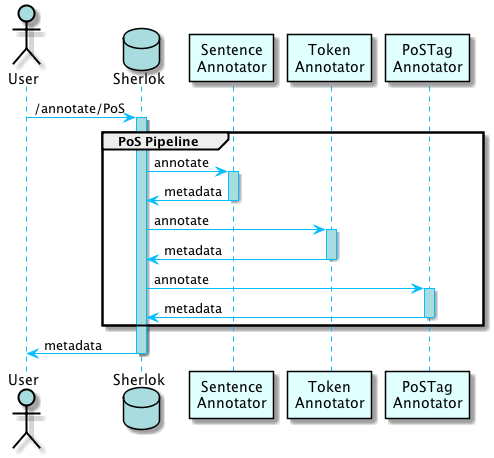
\includegraphics[width=0.7\linewidth]{res/sherlok_basic_rest_call.png}
    \caption{Part of Speech Pipeline}
    \label{fig:sherlok_basic_rest_call}
\end{figure}

\subsection{UIMA-Based Configurable Service}

Internally, Sherlok processes the input text through Unstructured Information Management
Architecture (UIMA)~\cite{uima} engines or more generally through a Rule-based Text Annotation
(RUTA) scripts~\cite{ruta}~\cite{ruta_2014}. Both RUTA and UIMA are projects of the Apache Software
Foundation \cite{apachefundation} focusing in analysing large volumes of unstructured information in
order to discover knowledge that is relevant to an end user. While Sherlok focuses on the Java
Frameworks for UIMA, it could be extended in the future to also support the C++ or Scaleout
Frameworks.

In order to let users who are not Java developers combine engines together, Sherlok has a Java
agnostic configuration system that separate the definition of engines from their usage in pipelines.

Those configuration files make use of two concepts:

\begin{description}
    \item[Bundles] The user lists the UIMA engines that he wants to use in \emph{bundles} by
        specifying the Java package dependencies, the required resource files and configure the
        different parameters of the engines. To simplify installing resources, Sherlok supports
        download at execution time of Git repositories or HTTP(S) URLs, but also lets the user
        specify local path on the server if needed.
    \item[Pipelines] The user writes the RUTA script which can be as simple as chaining engines from
        the bundles configuration files in \emph{pipelines}. The whole features set of RUTA is
        available to the user so that simple scripts don't require any Java implementation from the
        user. Similarly to bundles, Sherlok allow downloading resources for pipeline automatically.
\end{description}

By default Sherlok comes with pipelines to extract information about brain regions, part of speech
and much more. The engines used in those pipelines come from bluima, which is presented in Section
\ref{sec:bluima}.

The annotations produced by a pipeline are returned from the server in JSON format~\cite{json}. For
example, Listing~\ref{lst:json_sententence_detection} highlights the annotations in JSON format
produced by the \ID{bluima.sentence} pipeline when processing ``\textit{Terminologies which lack
semantic connectivity hamper the effective search in biomedical fact databases and document
retrieval systems. We here focus on the integration of two such isolated resources, the term lists
from the protein fact database UNIPROT and the indexing vocabulary MESH from the bibliographic
database MEDLINE.}''

In this listing are displayed three annotations: one \ID{DocumentAnnotation}, which provides insight
on the language of the processed document, and two \ID{Sentence}, each of which have a general
\ID{componentId} representing which NLP component has been used to derive the annotation.
Additionally, all three annotations have information about the corresponding range of the text that
they cover.

% The following listing is too big to fit properly. Also there are so many things that are not
% really interesting for the reader.
%\begin{lstlisting}[language=json,firstnumber=1]
%{"_context" : {
    %"_types" : {
      %"DocumentAnnotation" : {"_id" : "uima.tcas.DocumentAnnotation",
        %"_feature_types" : {"sofa" : "_ref" } },
      %"Sentence" : {"_id" : "de.julielab.jules.types.Sentence",
        %"_feature_types" : {"sofa" : "_ref" } },
      %"Sofa" : {"_id" : "uima.cas.Sofa",
        %"_feature_types" : {"sofaArray" : "_ref" } },
      %"Annotation" : {"_id" : "uima.tcas.Annotation",
        %"_feature_types" : {"sofa" : "_ref" },
        %"_subtypes" : ["DocumentAnnotation",  "Annotation" ] },
      %"AnnotationBase" : {"_id" : "uima.cas.AnnotationBase",
        %"_feature_types" : {"sofa" : "_ref" },
        %"_subtypes" : ["Annotation" ] },
      %"TOP" : {"_id" : "uima.cas.TOP",
        %"_subtypes" : ["AnnotationBase",  "Sofa" ] },
      %"Annotation" : {"_id" : "de.julielab.jules.types.Annotation",
        %"_feature_types" : {"sofa" : "_ref" },
        %"_subtypes" : ["Sentence" ] } } },
  %"_views" : {
    %"_InitialView" : {
      %"DocumentAnnotation" : [
        %{"sofa" : 1,  "begin" : 0,  "end" : 328,  "language" : "en" } ],
      %"Sentence" : [
        %{"sofa" : 1,  "begin" : 0,  "end" : 135,  "componentId" : "de.julielab.types.OpenNLPSentenceDetector" },
        %{"sofa" : 1,  "begin" : 136,  "end" : 328,  "componentId" : "de.julielab.types.OpenNLPSentenceDetector" } ] } },
  %"_referenced_fss" : {
    %"1" : {"_type" : "Sofa",  "sofaNum" : 1,  "sofaID" : "_InitialView",  "mimeType" : "text",  "sofaString" : "Terminologies which lack semantic connectivity hamper the effective search in biomedical fact databases and document retrieval systems. We here focus on the integration of two such isolated resources, the term lists from the protein fact database UNIPROT and the indexing vocabulary MESH from the bibliographic database MEDLINE." } } ,
  %"_stats" : {
    %"_pipeline_resolution": 3285,
    %"_annotation": 435
  %}
%}
%\end{lstlisting}

\begin{lstlisting}[float,language=json,
                   caption=Excerpt of JSON output for sentence detection,
                   label=lst:json_sententence_detection]
"DocumentAnnotation" : [
  { "begin" : 0,    "end" : 328,  "language" : "en" }
],
"Sentence" : [
  { "begin" : 0,    "end" : 135,
    "componentId" :
        "de.julielab.types.OpenNLPSentenceDetector" },
  { "begin" : 136,  "end" : 32
    "componentId" :
        "de.julielab.types.OpenNLPSentenceDetector" }
]
\end{lstlisting}

For quality purpose, Sherlok also allows the user to embed tests for pipelines that can be run
through the \REST{GET /test/<pipeline>} query in order to ensure that pipelines continue to work
properly after updating Sherlok or the engines' dependencies.

\section{Bluima, UIMA and RUTA}
\label{sec:bluima}

Bluima is an open-source collection of UIMA readers~\cite{uima} augmented by multiple engines
developed at the Blue Brain Project~\cite{bbp} to perform large-scale information extraction from
the neuroscientific literature. It includes for example a species annotator based on the Linnaeus
library~\cite{linnaeus_2010}, or the OpenNLP toolkit~\cite{opennlp} to perform Part of Speech
tagging, sentence splitting and more. Table~\ref{tab:bluima_subprojects} lists the major subprojects
used by bluima annotator engines.

\begin{table}[h]
    \centering
    \begin{tabularx}{\tablewidth}{@{} l Y @{}} % no margin at extremum
        \toprule

        OpenNLP~\cite{opennlp} & A machine learning based toolkit for the processing of natural
        language text. \\

        \midrule

        Linnaeus~\cite{linnaeus_2010} & A general-purpose dictionary matching
        software, capable of processing multiple types of document formats in the biomedical domain.
        \\

        \midrule

        BANNER~\cite{banner_2008} & A named entity recognition system, primarily
        intended for biomedical text. \\

        \midrule

        Dragon Toolkit~\cite{dragon_2007} & A Java-based development package for academic use in
        information retrieval and text mining. \\

        \midrule

        BioAdi~\cite{bioadi_2009} & BioAdi identifies the mapping between SF (Short Form) and LF
        (Long Form) terms in paper. \\

        \midrule

        langdetect~\cite{langdetect} & A language detection library implemented in plain Java. \\

        \midrule

        JWI~\cite{jwi_2014} & A Java library for interfacing with Wordnet. \\

        \midrule

        jSRE~\cite{jsre_2006} & A Java tool for Relation Extraction. \\

        \midrule

        JULES~\cite{jules} & A collection of UIMA wrappers for OpenNLP. \\

        \midrule

        OSCAR4~\cite{oscar_2011} & An open source extensible system for the automated annotation of
        chemistry in scientific articles. \\

        \bottomrule
    \end{tabularx}
    \caption{bluima aggregated projects}
    \label{tab:bluima_subprojects}
\end{table}

UIMA-based applications are structured into components called \emph{analysis engines}, or
\emph{annotators}, which produce metadata in form of annotations. The implementation of such engines
can be either written in C++ or in Java, however C++ development seems rather marginal compared to
the amount of available libraries and tool for UIMA in Java, for which several implementation
strategies have been devised over the years. The most modern and popular API used to build
components is \emph{uimaFIT}~\cite{uimafit}~\cite{uimafit_2009}: it aims to simplify the archaic XML
description used in earlier UIMA APIs to configure (C++ or Java) engines by writing both the
implementation and configuration of engines' parameters directly in Java. While Sherlok is
compatible with any UIMA-compatible technology, we focus on the uimaFIT approach in what follows.

At runtime, an annotator has mainly two actions: initialisation and processing. Annotations produced
by engines is stored in a Common Analysis System (CAS)~\cite{cas} general purpose data structure,
which allows the representation of objects with single-inheritance hierarchy, properties and values.
And in a pipeline of annotators, a single CAS instance is passed from one engine to the next so that
the data from previous engines can be used to filter data, augment existing annotations or produce
new ones.

Figure~\ref{fig:pos_pipeline_uimafit} depicts how uimaFIT-based applications handle pipelines such
as PoS tagging: first, the text to be processed is loaded into a CAS instance, then engines are
created through uimaFIT factory system with the appropriate configuration settings and finally the
pipeline of engines is run.

\begin{figure}[h]
    \centering
    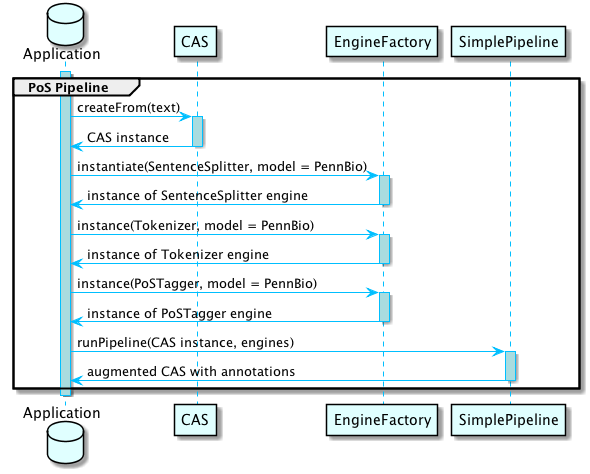
\includegraphics[width=0.9\linewidth]{res/uimafit.png}
    \caption{Part of Speech tagging uimaFIT pipeline}
    \label{fig:pos_pipeline_uimafit}
\end{figure}

While uimaFIT is very convenient when writing an UIMA application that is entirely written in Java,
it becomes much more complex when we want to include a flexible external configuration as we do with
Sherlok. Moreover, and especially for simple pipelines, sometimes implementing a Java annotator
requires more boilerplate code than the actual algorithm.

To workaround this, an application can use the RUTA language~\cite{ruta}~\cite{ruta_2014}, which is
an imperative rule language extended with scripting elements that can also be used to define
pipelines. To illustrate this, Listing~\ref{lst:ruta_example_dog} shows a very simple script that
annotates ``dog'' as an ``Animal'' and Listing~\ref{lst:ruta_example_pos} shows how RUTA can be used
to run the PoS pipeline from Figure~\ref{fig:pos_pipeline_uimafit}. For this last example, unlike
with uimaFIT, the XML description of engines' parameters need to be available at runtime as it is
not embedded in the script itself.

\begin{lstlisting}[float,language=ruta,
                   caption=A basic RUTA script,
                   label=lst:ruta_example_dog]
DECLARE Animal;
W{REGEXP("dog") -> MARK(Animal)};
\end{lstlisting}

\begin{lstlisting}[float,language=ruta,
                   caption=PoS pipeline written in RUTA,
                   label=lst:ruta_example_pos]
ENGINE SentenceAnnotator;
ENGINE TokenAnnotator;
ENGINE PosTagAnnotator;

Document{-> EXEC(SentenceAnnotator)};
Document{-> EXEC(TokenAnnotator)};
Document{-> EXEC(PosTagAnnotator)};
\end{lstlisting}

Fortunately, uimaFIT provides tools to generate XML descriptions for classic engines so that we can
use RUTA to generate pipeline automatically for the user from a simpler description of the engines'
parameters than raw XML as follows:

\begin{enumerate}
    \item the user defines the engines with their parameters inside bundles;
    \item then he defines the order of engines in a given pipeline;
    \item when the user wants to annotate a given text with the pipeline, Sherlok converts the
        engines, with their configured parameters, used by the pipeline into XML descriptions;
    \item Sherlok generates a RUTA script that uses the engine descriptions in the order of the
        pipeline;
    \item and finally, Sherlok runs the RUTA script and return the annotations back to the user.
\end{enumerate}

Additionally, Sherlok allows users to use the full RUTA language in pipelines to create even more
powerful tools. And in order to make configuration more flexible, as we will see in Section
\ref{sec:config_in_sherlok}, the user has the possibility to user configuration variables in bundles
or pipelines to download automatically remote resources.

\section{Packaging Strategy}
\label{sec:packaging2}

Initially all resources used by bluima's engines, such as models trained on the GENIA corpus
\cite{genia} to tag part of speech elements, were accessed via a system wide path variable. In this
section we will discuss the adopted strategy to improve this system and make bluima
``path-agnostic'' in order to improve its integration in Sherlok. In the
Appendix~\ref{sec:packaging1} we show a few other alternatives that were also considered during this
project.

\subsection{Initial Situation}

Both bluima and Sherlok build system are based on Apache Maven~\cite{maven}, which allows developers
to define how a Java project should be compiled, packaged, tested and much more. One important
feature of Maven is its ability to download dependencies from centralised repositories where
developers can publish their releases. At the beginning of this project, however, bluima was not yet
available in Maven central which meant that to use it one had to clone its Git repository, compile
and install it.

Yet, publishing bluima to Maven Central would not suffice to solve a bigger issue. Bluima widely
uses resource files in its engines and therefore needs to access those files at runtime. Originally,
it used a system global variable (\VAR{BLUIMA\_HOME}) as many popular tools do nowadays (e.g. Java
with its \VAR{JAVA\_HOME}) to locate specific files. Thus, using Maven to download and install Java
archives (\JAR) is not enough to locate those files later at runtime: the variable must be set at a
system-wide level by the user itself.

This made it clear that we needed a better engines-resources model or the integration of bluima in
Sherlok would imply that system administrators would have to manually install and configure bluima,
which in itself would defeat the whole purpose of Sherlok to make users' life better and automate
dependencies installation.

\subsection{Proposed Solutions}

There exist, as always, many methods to address this issue. But for this project, in addition to
ease the integration of bluima in other tools, we wanted to keep the refactoring and maintenance
cost low, allow resources to refer to one-another, make it possible to group files together in
\emph{batches}, avoid runtime performance penalties wherever possible and remove as little
flexibility from the users as possible.

\subsubsection{Refactoring and Maintenance}

The first idea that we explored was to package resources inside \JAR files and use Maven to
distribute them similarly to what DKPro~\cite{dkpro}~\cite{dkpro_2014} does but in a less complex
manner for the users.

In a nutshell, packaging resources within \JAR files has two important drawbacks. Firstly, updating
a resource file implies repackaging and redeploying the new version to, for example, Maven Central,
which can be quite a burden. One could argue that this is an administrative task that is not
frequent and therefore not significantly enough to discard this strategy. However, the second issue
is of much more concern.

As detailed in appendix~\ref{sec:packaging1}, this packaging strategy implies more refactoring than
it seems at first sight: in order to be able to use an engine with different resources (e.g. one
might prefer to use a probabilistic tokenizer trained on the GENIA corpus to process some inputs,
but use a model trained on a different corpus for some other inputs) and not hardcode them, we need
a \emph{proxy} to select from an identifier the appropriate files at runtime.

In appendix~\ref{sec:packaging1}, we illustrate this with a technique using as the identifier the
name of the class that ``owns'' the desired resource file. Although the fact that the implementation
of the proxy we designed is based on the Java Reflection API is not related to the amount of
refactoring needed to adapt bluima to this packaging design, it significantly adds some complexity
to the overall software and therefore will increase its maintenance cost.

The Java API to access \JAR content is based on read-only access because, among other things, those
archives can be signed and thus modifying their content would threaten the integrity of the
signature or corrupt the archive.

The core refactoring issue with this design is that instead of working with \ID{File} objects or
paths as the initial implementation of bluima engines does, we would have to use \ID{InputStream} in
order to access the resources files because of how Java \JAR system was designed. And this can be
really problematic for some annotators. For example, the \ID{LinnaeusAnnotator}, which wraps the
external Linnaeus library~\cite{linnaeus}, uses an \ID{ArgParser} internally that cannot be created
from a data stream but absolutely requires a path to a configuration file.

Of course, some workarounds could be elaborated, such as copying the content of the file in the \JAR
file to a temporary file and then use this file's path, but only on a case by case basis and that
those would most probably induce performance penalties.

\subsubsection{Resource Interdependency}

The \ID{LinnaeusAnnotator} also illustrates another feature that engines might need: the ability to
reference a resource file from another resource file via relative paths. With DKPro-like solutions,
the usage of stream to read resources content makes it much harder to allow such behaviour.

Workarounds for this specific issue usually imply modifying the engines and their underlying
implementation to work differently. In the case of \ID{Linnaeus\-Annotator} this would have meant to
completely rewrite the Linnaeus library since it is a closed-source utility, which is clearly out of
the scope of this three-month project.

\subsubsection{Batch Of Files}

Like with \ID{LinnaeusAnnotator}, the \ID{BrainRegionPipes} use a batch of files: a collection of
configuration files used together to set up an annotator or its dependencies. For the
\ID{BrainRegionPipes} the problem is easier since no file makes a reference to another one.
Nevertheless, it would be very verbose and painful to denote each and every of the ~30 files one by
one in the configuration of the engine. Hence, considering a batch of files simply as a collection
of files without a specific naming structure is not optimal. Depending on whether or not we base the
resource packaging system on a system similar to DKPro, the consequences differ:

\begin{itemize}

    \item Were we to use a packaging strategy based on \JAR files, we could introduce an arbitrary
        naming structure for the identifiers used to access the actual resource through the proxy
        system and have an \emph{aggregator proxy} that generates multiple data streams to each and
        every individual resources from a single root identifier. While this solution seems simple
        on the paper it actually requires as much refactoring as using one identifier by resource.

        Additionally, it doesn't solve the interdependency between resources as illustrated above
        with \ID{LinnaeusAnnotator}.

    \item If we apply the idea of names having an arbitrary but constant structure to the filenames
        directly instead of the identifiers used by a proxy, we could group the resource files
        together in an archive (e.g. a zip file) that would get extracted at runtime into a
        temporary directory.

        With this approach we have at least two significant advantages over the \JAR-based design
        without sub-archives. Firstly, it only requires a minimal refactoring of the current Java
        code to extract and use the data as the implementation is based on \ID{File}s or
        \ID{String}s representing paths. Secondly, it allows files to refer to one another through
        relative paths.

        However, this would imply adding a relatively complex version checking system in bluima
        and/or Sherlok: in order to not extract data from an archive when it is already available to
        prevent degrading performance too much, we would have to check if the data was already
        extracted and if that's the case that it is actually correct. This can be quite complex
        when, for example, upgrading resources. And this is without mentioning having several
        pipelines using the same engine but with different version of its resources, nor dealing
        with multiple concurrent annotation instances. Finally, if we take the example of Sherlok
        running on several servers, we introduce an issue of data accessibility and replication for
        cache purposes.

\end{itemize}

\subsubsection{Flexibility}

With all the above issues, the \JAR-based packaging design seems rather inconvenient to use, mainly
because it involves a lot of refactoring. Moreover it adds some complexity to the implementation.
Some engines behave differently depending on the file type of some of their resources: for example,
the \ID{SuffixSensitiveGISModelReader} utility reads the content of its input resource differently
depending if the file extension is ``\PATH{.bin}'' or ``\PATH{.txt}''. When using \ID{InputStream}
instead of \ID{File} the extension is lost and therefore need to be tracked with an additional
parameter.

In addition to all the above issues, we could argue that we actually remove flexibility from the
users by forcing them to use a Java system to archive and manage resources despite the fact that the
system using bluima could be Java agnostic from the final user point of view. It could actually be
quite painful for someone who is using a Source Control Management (SCM) tool, such as Git, to
manage two distinct files structures: one that is convenient to the user and one for our \JAR-based
archiving system.

Moreover, if we take the example of batch of files, at the end of the day, we have extracted some
data that the user had to package initially in order to make the installation process easy but
incredibly complexify the implementation.


\subsubsection{Adopted Solution}

We argue that the installation process for runtime resources could be much simpler than packaging
resources into \JAR files in the first place, potentially aggregating batch of files together in
sub-archives, then accessing those files via a proxy and an extra layer of resource identifiers,
potentially extracting sub-archives into a temporary directory, and by this mean forcing the user to
use a specific versioning system as DKPro-like systems do.

The \JAR-based system that we present in Appendix~\ref{sec:packaging1} can, if needed, add an
additional runtime safety by ensuring that resources are present. However, we argue that this
additional security layer is not really necessary since it is rather trivial to detect a missing
file from an engine at runtime and propagate an error to the user, but also because this kind of
situation should not occur at all once the pipelines have been tested. Moreover, we can directly
make some basic checks in Sherlok that are in practice sufficient. For these reasons we don't
consider it as a critical downside.

From bluima perspective, the user could simply install the configuration files in a directory of his
choosing and configure the engines with paths to the actual resources without using any system-wide
variable. Withal, since this simpler approach does not enforce any versioning mechanism at all, the
user is free to implement any system that matches his needs. Following from this fact, Sherlok can
add an extra layer, directly integrated in the bundle \& pipeline configuration files, to manage
resources easily for the end users. Such system can, but is not restricted to, be based on Git: a
user can define a (batch of) resource(s) by a Git repository and an optional tag or commit SHA and
Sherlok then can automatically download and install the specific version of the resources.

This last solution allies the flexibility of using Java \ID{File} objects, and therefore involves
only little refactoring of bluima annotators, with the power of external, well-establish and
powerful SCM tools in addition to avoid the limitation of having to rely solely on \ID{InputStream}
to access resources. This is why it was selected and implemented in this project.

We present in Table~\ref{tab:packaging_strategies} a quick summary of the pros and cons of all the
techniques we have explored for this project. The four ``\emph{proxy-based}'' versions are detailed
in Appendix~\ref{sec:packaging1}. The first column reports the workload needed to implement and use
the corresponding approaches in bluima. The second one indicates if the code can be constructed in a
concise way (DRY standing for \emph{Don't Repeat Yourself}). The flexibility column tells how easy
it is for users to integrate their resources. The fourth one represents the amount of work needed to
propagate a new version of some resources to the packaging system. And finally the last one states
whether or not the system integrates a runtime safety net.

\begin{table}[h]
    \centering
    \begin{tabular}{l c c c c c}
        Strategy & \VERTICALTEXT{Refactoring-Friendly}
                 & \VERTICALTEXT{DRY-code}
                 & \VERTICALTEXT{Flexibility}
                 & \VERTICALTEXT{Repackaging Cost}
                 & \VERTICALTEXT{Runtime Safety} \\

        \toprule

        DKPro-Like~\cite{dkpro} & \XMARK & \CMARK & (\CMARK) & \XMARK & \XMARK \\

        \midrule

        Proxy-Based A & \XMARK & \CMARK & \XMARK & \XMARK & \CMARK \\

        \midrule

        Proxy-Based B & \XMARK & \CMARK & \XMARK & \CMARK & (\CMARK) \\

        \midrule

        Proxy-Based C & \XMARK & \XMARK & \XMARK & \XMARK & \CMARK \\

        \midrule

        Proxy-Based D & \XMARK & \CMARK & \XMARK & \CMARK & \XMARK \\

        \midrule

        Adopted Solution & \CMARK & \CMARK \CMARK & \CMARK \CMARK & \CMARK & \XMARK \\

        \bottomrule
    \end{tabular}
    \caption{Packaging Strategies Comparison}
    \label{tab:packaging_strategies}
\end{table}

\subsection{Impact on bluima}

One of the important aspect of the adopted solution is that it is actually easy to implement: bluima
only need some minor refactoring and it can be extended to other project easily, regardless of their
implementation language or tools.

Because we now want to work only with generic paths, the refactoring mostly consists in adding
configuration parameters to annotators to handle custom resource locations. For example, the
\VAR{modelFile} parameter of \ID{Sentence\-Annotator}, which represents the model to use for
detecting sentences, should be capable of loading a file from wherever on the disk.

Usually this refactoring is trivial: we only need to introduce an extra parameter to compute paths
to files or directories. And since this only adds flexibility, we don't see any downside to this
technique.

However, this implies that a marginal part of the current code base of bluima needs to get upgraded,
deprecated or even removed. For example, the \ID{OpenNlp\-Helper} class is a utility to load NLP
annotators, such as \ID{Sentence\-Annotator}, and configure them with the models trained on the
PennBio corpus. But since this utility uses a fixed path, based on the global variable
\VAR{BLUIMA\_HOME}, to locate model resources, it cannot be used as-is. For this specific case, it
is easier to simply deprecate it for mainly two reasons:
\begin{enumerate*}[label=\itshape\alph*\upshape)]
    \item using the NLP annotators directly is straightforward;
    \item and more importantly, this factory is not compatible with RUTA and Sherlok scripting system.
\end{enumerate*}

Additionally, unit tests need to be refactored to take into account that using the
\VAR{BLUIMA\_HOME} environment variable is no longer reliable. Fortunately, this is rather trivial
for bluima since its build system is Maven: unit tests can be configured through the
\ID{maven-surefire-plugin} at compile time, without any user interaction, to set a Java property
that represent the root directory of all bluima resources. Then, the refactoring of tests is as
simple as using the newly introduced Java property instead of a system-wide variable.

Finally, because annotators are now independent of the location of their resource files, we can move
the resources into a separate Git repository and include it in bluima with a Git submodule. As we
will see in the Section~\ref{sec:config_in_sherlok}, this has the nice property of allowing Sherlok
to download only those resources at runtime, and thus spare the effort of downloading the full
bluima code base which weighs more than 700MB (with its history).

\subsection{Configuration in Sherlok}
\label{sec:config_in_sherlok}

Now that we have system that allows resources to be located anywhere on the filesystem and used at
runtime, we can go further and propose a flexible integration system for resources in Sherlok.

We can use the fact that resources are identified when configuring annotators to let Sherlok
download them automatically on-demand, similarly to regular Maven dependencies for the actual
annotator implementation. To do that, we add the ability to define and use \emph{configuration
variables} in bundles and pipelines that will, after the resources have been downloaded to an
internal directory of Sherlok, be substituted by the actual path to the corresponding resources.

For example, Listing~\ref{lst:sentence_annotator_config} shows how the \ID{SentenceAnnotator} engine
can be defined in a bundle with
\begin{enumerate*}[label=\itshape\alph*\upshape)]
    \item its Java dependencies using Maven artefacts (here the only dependency is
        \ID{bluima\_opennlp} which contains the Java class \ID{ch.epfl.bbp.uima.ae.SentenceAnnotator});
    \item and its runtime resources (here the trained model \PATH{SentDetectGenia.bin.gz} from the
        master branch of \ID{bluima\_resources} Git repository).
\end{enumerate*}

\begin{lstlisting}[float,language=json,
                   caption=Configuration of \ID{SentenceAnnotator} in a Sherlok bundle,
                   label=lst:sentence_annotator_config]
{
  "name": "bluima.sentence",
  "domain": "examples",
  "version": "1.0.1",
  "dependencies": [
    {
      "value": "ch.epfl.bbp.nlp:bluima_opennlp:1.0.1"
    }
  ],
  "config": {
    "bluima": {
      "type": "git",
      "url":
        "https://github.com/BlueBrain/bluima_resources.git",
      "ref": "master"
    }
  },
  "engines": [
    {
      "name": "SentenceAnnotator",
      "class": "ch.epfl.bbp.uima.ae.SentenceAnnotator",
      "parameters": {
        "modelFile": [
          "$bluima/opennlp/sentence/SentDetectGenia.bin.gz"
        ]
      }
    }
  ]
}
\end{lstlisting}

When defining a pipeline in Sherlok that uses RUTA scripting elements, users might want also to
fetch runtime resources as well. Therefore, we added the same ability to define configuration
variables inside pipelines. Moreover, Sherlok is capable of downloading remote resource over HTTP as
shown in Listing~\ref{lst:countries_pipeline_config} where a list of countries is downloaded when
the pipeline is used. The only particularity with resources that are used directly in RUTA scripts
is that they need to be in a special mode because the underlying path needs to be computed slightly
differently.

\begin{lstlisting}[float,language=json,
                   caption=Configuration of the \ID{countries} pipeline,
                   label=lst:countries_pipeline_config]
{
  "name": "countries",
  "version": "1",
  "description": "Example that annotates countries",
  "domain": "examples",
  "config": {
    "countries": {
      "type": "http",
      "url": "https://example.com/countries.txt",
      "mode": "ruta"
    }
  },
  "script": [
    "WORDLIST CountriesList = '$countries';",
    "DECLARE Country;",
    "Document{-> MARKFAST(Country, CountriesList)};"
  ]
}
\end{lstlisting}

Yet, downloading remote resources can be costly and should only be done when the resources are
needed and not repeated unless needed. This is why Sherlok will cache resources once they have been
fetched the first time they are used. Conversely, keeping resources that are not used can be costly
for the system administrators. Hence why they can be removed through REST calls, such as \REST{DELETE
/clean/runtime\_resources} that will remove any downloaded resources.

Additionally to Git and HTTP configuration variables, Sherlok also supports basic text variable and
is designed to be easily extended to support more type of remote resources, such as SVN or Mercurial
repositories, remote files over SSH or any other communication protocol.

To support a new protocol, Sherlok code base needs to be extended as follows:

\begin{enumerate}
    \item a new class implementing the \ID{ConfigVariable} Java interface and supporting the new
        protocol needs to be created;
    \item the \ID{ConfigVariableFactory.factory} method needs to be augmented to create the new kind of
        variable when appropriate;
    \item and, optionally, the \ID{ConfigVariableFactory.cleanerFactory} method can be extended to
        support cleaning resources of the new kind.
\end{enumerate}

And to conclude this section, Figure~\ref{fig:sherlok_load_pipeline} depicts how bundles and pipelines
are combined together to generate the underlying RUTA script that Sherlok will use to annotate text.

\begin{figure}
    \centering
    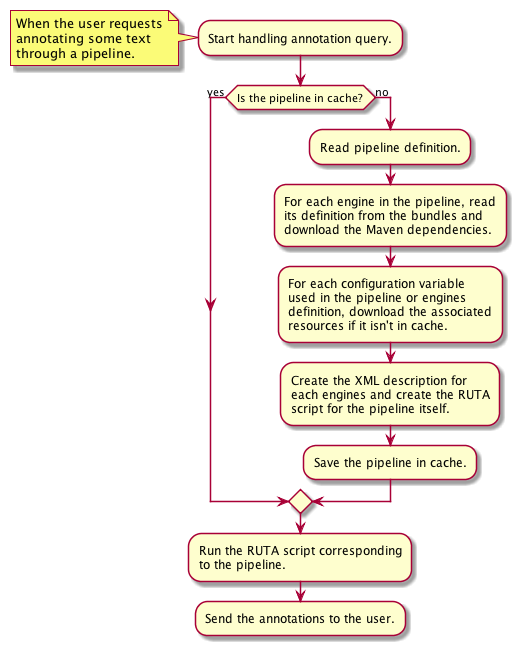
\includegraphics[width=\linewidth]{res/sherlok_load_pipeline.png}
    \caption{Sherlok pipeline loading procedure}
    \label{fig:sherlok_load_pipeline}
\end{figure}

\subsection{Possible Extensions}
\label{sec:config_variable_extensions}

The implementation of the previous concept in this project proves that this strategy works well for
Sherlok. But yet users might want more features, such as more remote protocol support (SVN, hg, SSH,
\dots) as previously mentioned. Here we list a few other features that could be interesting to
implement.

\begin{description}

    \item[Archive Extraction] When working with batch of files, it can be convenient to download an
        archive and extract it automatically. This could be easily be added to Sherlok by adding a
        parameter for the HTTP configuration variable.

    \item[Redownload If Newer] Being able to fetch remote files, especially with HTTP protocol, is
        very useful. Currently, once resources have been downloaded and cached by Sherlok they won't
        be redownloaded until they are cleaned. Therefore, if the remote resource is updated, the
        system administrator has to clean it manually. However, this could be easily be improved by
        supporting automatic update of HTTP resources by using the \ID{If-Modified-Since}
        request-header field.

    \item[Pull Git Branch] Sherlok currently supports selecting specific commit, branch or tag in
        configuration variable when working with Git repositories. But similarly to HTTP resources,
        once the data has been fetched and cached it won't be updated until it has been clean. It
        would be convenient to get automatic update from upstream. This could either be simply
        implemented by pulling the new history at periodic intervals, or by using web hooks or
        equivalent techniques. But Sherlok would have to be very careful and do it only when the
        resources are not in use by any pipeline or it would risk corrupting running engines.

    \item[Improve Download Strategy] While the current implementation works well, there are a few
        area that could benefit from optimisation. For example, naively cloning the whole Git
        repository with its complete history only to checkout a specific commit or tag is really
        under-efficient. Instead, for this specific case, downloading only the most recent history
        from the server is much faster. This can be archived with the ``\verb#--depth 1#'' option of
        Git command line.

\end{description}

\section{Conclusion \& Future Development}
\label{sec:conclusion}

With this project we have shown that Sherlok can be used to write pipelines for general NLP
processing. For example, we were able to create a simple pipeline to detect sentences, but more
conclusively we also have created a full brain region detection pipeline, based on
jSRE~\cite{jsre_2006}, that is displayed in Listing~\ref{lst:brain_region_pipeline_jsre}.
Furthermore, we have derived this pipeline into two variants: one using a top-down approach, the
other using a rule-based approach.

\begin{lstlisting}[float,language=json,
                   caption=jSRE brain region pipeline,
                   label=lst:brain_region_pipeline_jsre]
{
  "name": "bluima.regions_jsre",
  "version": "1.0.1",
  "description": "annotate brain regions",
  "domain": "bluima",
  "script": [
    "ENGINE SentenceAnnotator:1.0.1;",
    "ENGINE TokenAnnotator:1.0.1;",
    "ENGINE PosTagAnnotator:1.0.1;",
    "ENGINE BlueBioLemmatizer:1.0.1;",
    "ENGINE MeasureRegexAnnotator:1.0.1;",
    "ENGINE PruneMeasuresAnnotator:1.0.1;",
    "ENGINE LinnaeusAnnotator:1.0.1;",
    "ENGINE BrainRegionAnnotator:1.0.1;",
    "ENGINE KeepLargestBrainRegionAnnotator:1.0.1;",
    "ENGINE ExtractSameBrainRegionCoocurrences:1.0.1;",
    "ENGINE JsreBrainRegionFilterAnnotator:1.0.1;",
    "ENGINE KeepLargestCooccurrenceAnnotator:1.0.1;"
  ]
}
\end{lstlisting}

A fourth technique to detect brain regions is based on \ID{ConceptMapper} from UIMA Addons and
Sandbox~\cite{uima_sandbox}. \ID{ConceptMapper} is defined as follows in its documentation:

\begin{quotation}
    [It] is a highly configurable, high performance dictionary lookup tool, implemented as a UIMA
    component. Using one of several matching algorithms, it maps entries in a dictionary onto input
    documents, producing UIMA annotations.
\end{quotation}

However, it is not directly compatible with Sherlok bundle and pipeline system as it is already in
itself an abstraction over UIMA components. Nevertheless, we believe that some mechanism could be
set up to accommodate the integration of this powerful tool into Sherlok.

The challenge would be to make users able to express in bundles and pipeline descriptions their
intention to use \ID{ConceptMapper}, which basically takes as input a XML file containing
essentially:
\begin{enumerate*}[label=\itshape\alph*\upshape)]

    \item the configuration parameters description;

    \item the configuration parameters values;

    \item the UIMA type system for annotations.

\end{enumerate*}
The first point could be abstracted with a uimaFIT engine written in Java and the second correspond
to the configuration of such engine in a bundle. The third one could be extrapolated from Sherlok's
knowledge of the different engines used in a pipeline or provided by the user.

However, the tricky part is that one of the configuration parameters of \ID{ConceptMapper} is a XML
description of a tokenizer to interpret data from the input dictionary. Since this description can
be generated from a uimaFIT engine, one could devise a mechanism in Sherlok to automatically
generate it from a selected tokenizer engine with some special syntax in bundle configuration.

On a different topic for improvement, and independently of the extensions mentioned in
Section~\ref{sec:config_variable_extensions}, one could make Sherlok capable of downloading the text
that the user wants to annotate through common protocol such as HTTP or SSH: instead of using
\REST{GET /annotate/<pipeline>?text=<input>}, we could imagine that users would specify the remote
URL where the text is hosted with, for example:

\[
    \REST{GET /annotate/<pipeline>?ssh=<url>}
\]

Additionally, Sherlok and bluima could be extended to fully support input in different format, such
as PDF or HTML. This is possible by using special engines, called text adaptor, at the beginning of
the pipelines that would extract the actual text from the input file and pull out the interesting
metadata for the user. Those text adaptors could extract more than just the raw text. For example, a
PDF extractor could include information about text emphasis, whether a word is part of a section
title, if proper name is an author or replace images by a text description.

\clearpage
\begin{appendices}

\section{Proxy-Based Packaging Strategy}
\label{sec:packaging1}

The initial idea was to base the system on Apache Maven~\cite{maven}. However, while implementing the
strategy described below we realised that it was not as flexible as predicted. A better alternative
is presented in Section~\ref{sec:packaging2}. This section describes our first approach.

One of the first objective of this project was the disassociation of algorithms (engine annotators)
and their different resources (model files, configuration files) and devise a packaging system,
based on Apache Maven, that would be flexible while being simple and convenient to use and let the
user define pipelines using specific annotators and models.

\subsection{Packaging}

With Maven, main idea is to store a set of resources, such as dataset trained on a specific corpus
of texts, in a \JAR file and access them in read-only mode at runtime. And after the packaging of
resources is done, the {\JAR}s are published on a public repository such as Maven Central. Then
package dependencies can be used to ensure that some files are available at runtime. And, ideally,
package versions should be used to let users update resources independently of the algorithms.

Tools like DKPro~\cite{dkpro} already provide method to ship resource alongside algorithm. However,
we decided to use a different system because DKPro is rather complex, although flexible, and because
it heavily relies on ANT scripting build system to export data into \JAR files, which is not
straightforwardly integrable into Maven build system.

It might not be clearly apparent for someone not used to work with Java \JAR-based system, but with
this approach we cannot modify the resource files at runtime since they have been packaged, and this
for mainly two reasons. Firstly, the Java API doesn't provide standard tools to modify such
archives. And secondly, if the \JAR file were signed (which is the standard procedure) then
modifying its content would actually break the signature and therefore corrupt the archive.

Additionally, the API to access resources inside \JAR files is not based on Java \ID{File} objects.
Instead algorithms have to use \ID{InputStream} objects through \ID{ClassLoader} objects to access
the content of a given file. We will discuss how the current code need to be refactored in
Section~\ref{sec:restructuring_bluima}.

Here we describe three alternatives that we used to contrast alternative strengths and weaknesses
before concluding with a fourth variant that should match our needs. Below, \ID{ada} and \ID{bob}
denote two variants of a kind of resource that are compatible with a common algorithm package,
denoted \ID{algo}. The \ID{using*} packages can be thought of as pipelines in the context of
bluima/Sherlok.

\subsubsection{Proxy-Based: Version A}

The first system we analysed spread each algorithm and set of resources into individual packages
that depends on \ID{modeldep}, a proxy utility to access the resource files inside \JAR files. If an
algorithm depends on some resource file then it accepts as input parameter the model name (as a
string) and uses the proxy to load the file. In this scenario pipeline packages have dependencies
toward their annotators but also toward specific models as shown in Figure~\ref{fig:pkgsysA}.

This system has several positive aspects. First of all, tests can be easily written by specifying
potentially multiple resource packages as dependencies with Maven's test scope. Then, \ID{modeldep}
also defines a clear Java interface to define the contract for models and their versions.
Additionally, the proxy system centralises the utility to load resources and therefore eases
maintenance by not involving code duplication in several packages. However, models could not be
swapped on the fly since it would involve recompiling and repackaging \ID{using\_my\_algo}.
Alternatively, to prevent modifications, \ID{using\_my\_algo} could depend on both \ID{ada} and
\ID{bob} packages but this would not be as flexible as we want it to be.

\begin{figure}
    \centering
    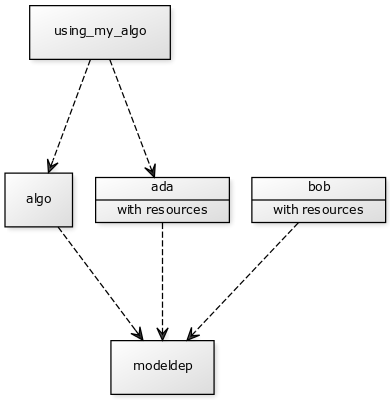
\includegraphics[width=200pt]{res/packaging_version_A.png}
    \caption{Proxy-based packaging system, version A}
    \label{fig:pkgsysA}
\end{figure}


\subsubsection{Proxy-Based: Version B}

The second approach is based on Maven's version string: an \ID{algo} will depend on an abstract
\ID{model} which provides a mechanism to load a specific file from its \JAR file and both \ID{ada}
and \ID{bob} model versions are defined as subversion of \ID{model}. For example, the convention
could be that if \ID{model} is defined as version \ID{0.1} then \ID{ada} will use the string
\ID{0.1-ADA} to define its version and the \ID{algo} will accept versions in the range $ [0.1,0.2)
$.

The model actually used will be either specified at compile time (cf. \ID{using.algo2}) or be
selected at runtime depending on the installed packages (cf. \ID{using.algo1}) as depicted on
Figure~\ref{fig:pkgsysB}. While this offers a great flexibility to the user designing pipelines and
allows him to swap models without repackaging anything, it means that test projects cannot ensure
the correctness of more than one model version at a time. Moreover, if no specific version is bound
to the pipeline, such as with \ID{using.algo1}, then there is no strong guarantee that a valid
version is available at runtime.

\begin{figure}
    \centering
    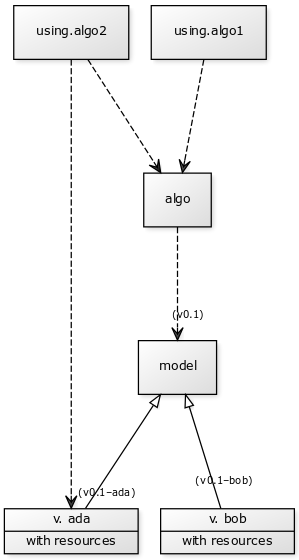
\includegraphics[width=200pt]{res/packaging_version_B.png}
    \caption{Proxy-based packaging system, version B}
    \label{fig:pkgsysB}
\end{figure}


\subsubsection{Proxy-Based: Version C}

The third version we studied is the most simple one: as illustrated on Figure~\ref{fig:pkgsysC},
instead of splitting everything in separate package, only annotators are packaged independently of
pipelines and resources, which are grouped together. On the one hand this system couldn't be simpler
but on the other, since pipelines often involve several engine annotators that are themselves used
in several pipelines, the coupling of models and the corresponding algorithm implies that many
packages have to be created to support each combination of models.


\begin{figure}
    \centering
    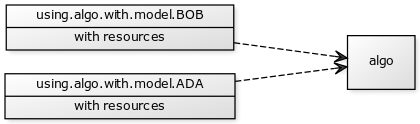
\includegraphics[width=200pt]{res/packaging_version_C.png}
    \caption{Proxy-based packaging system, version C}
    \label{fig:pkgsysC}
\end{figure}

\subsubsection{Proxy-Based: Version D}

After exploring possibilities offered by the Maven packaging system we analysed how resources and
engines are related to each others and used by pipelines in bluima. Figure~\ref{fig:pkgsysD} depicts
those relations. It was also considered that repackaging is an acceptable cost to swap models. The
most important point was avoiding at all cost to package an exponentially huge number of pipelines
to match each and every possible combinations and for this reason version C was discarded.

We also reflected on the structure of the algorithm, especially on their input arguments. We came to
the conclusion that, mostly for flexibility, they should accept \ID{InputStream}s as input and not
be bound to any models. Instead, the pipelines will be in charge to give them the proper resource
data streams. Therefore the pipeline will have dependencies toward algorithms and models.

Finally, in order to centralise code and simplify loading resources we introduce \ID{ModelProxy}, a
utility class used by pipelines that, given a \ID{String} representing a class name, opens a stream
to a given file inside the class' \JAR file.

In some cases, when processing the resource as a stream, it can be convenient to have access to its
original filename (e.g. when reading a compressed archive). Therefore we encapsulate the name and
the stream in a class -- \ID{ModelStream} -- that can be seen as a specialised \ID{InputStream} with
a filename property.

\begin{figure}
    \centering
    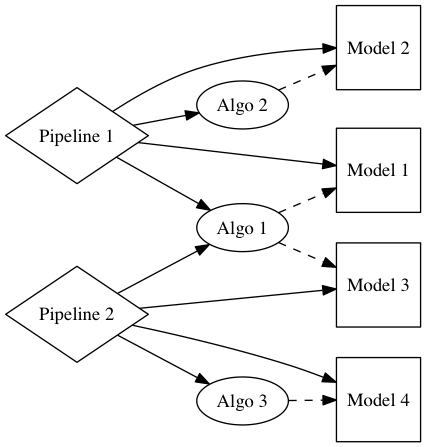
\includegraphics[width=200pt]{res/packaging_version_D.png}
    \caption{Proxy-based packaging system, version D}
    \label{fig:pkgsysD}
\end{figure}


\subsection{Restructuring bluima}
\label{sec:restructuring_bluima}

Now that the packaging strategy for annotators and their resources has been designed we can actually
apply it. It was decided to start with a relatively easy annotator --~Namely \ID{SentenceAnnotator}
which is part of OpenNLP~-- to make sure our previous decision was indeed viable. The approach was
based on an iterative process that can be applied to other modules as well. But before diving into
the details, we will first discuss how the different modules in bluima are related to each other.

We wanted to create a structured, yet flexible, file hierarchy for the annotators and their
resources. Since we are using Maven, we based our design on parent-child relationship in the
\ID{pom.xml} files: the root pom file, in addition to actually loading its children, defines the
main settings, such as the Java version to use or the list of general dependencies, that will be
shared with every of its children. The root pom file references both modules \PATH{modules/pom.xml}
and \PATH{resources/pom.xml} that are responsible for loading their own children, that is the
different annotators or utilities for the former and the actual resource for the latter.

It follows that when running the install (or test) command on the root Maven project then every
algorithms and resources are installed (or tested).

\subsubsection{Case Study: Converting OpenNLP}

When converting an annotator such as \ID{SentenceAnnotator}, the first thing to do is to identify
the unit test responsible for its quality. In this case, the annotator was converted from a classic
UIMA~\cite{uima} structure, based on XML description of engines and their configuration, to the more
modern structure defined by uimaFIT~\cite{uimafit}, which allows a more compact pipeline runner.

Once the unit tests are properly working, we move on to the generation of the resource packages.
Since this phase is completely repetitive, we devised a script to make the developer's live less
cumbersome: given a resource file, a resource name and a few other technical details we can produce
a resource package, as described previously, that is ready to be used with an annotator.

However, many annotators are currently using Java \ID{File} parameters, or Java \ID{String}s to
identify files on the local filesystem. Therefore, we have to refactor these annotators and their
dependencies in order to use \ID{ModelStream} instead. The following strategy was applied to convert
PoS, Token and Chunk annotator of OpenNLP:

\begin{enumerate}

    \item Renaming the \ID{PARAM\_MODEL\_FILE} parameter (or any similar properties) of the annotator
        into \ID{PARAM\_MODEL}.

    \item Updating its \ID{initialize} method to load a \ID{ModelStream} through \ID{ModelProxy} and the
        \ID{PARAM\_MODEL} parameter.

    \item Updating the annotator's dependencies such that they can be constructed from \ID{ModelStream}.
        Usually this plays well with the current implementation that must at some point use a
        \ID{FileInputStream}. Hence, we can plug in our custom stream in place of the regular
        \ID{FileInputStream} without restructuring the dependencies too much.

    \item Updating the dependency list in the annotator's \ID{pom.xml} file to reflect any additional
        resource dependency.

\end{enumerate}

Finally, at this last point the unit test should be updated to use resource package with
\ID{PARAM\_MODEL} instead of absolute path to the resource file.

However, as discussed in Section~\ref{sec:packaging2}, the third step is not always trivial or quick
to be implemented. The strategy defined in this section works well for relatively simple engines,
such as the one from OpenNLP, or for engines with a well-modularised implementation. But for
closed-source, more complex or engines with a defective software design that cannot withstand
refactoring easily, this task becomes much harder, if not close to impossible to implement.

\subsection{Configuration in Sherlok}

Listing~\ref{lst:sentence_annotator_config_old} illustrates how this strategy can then be used in
Sherlok bundles configuration. Compared to Listing~\ref{lst:sentence_annotator_config} from
Section~\ref{sec:config_in_sherlok}, here we have one extra Maven dependency
(\ID{bluima\_sentence\_detector\_genia}) which contains the essentially two things: the model file used
by \ID{SentenceAnnotator} and a proxy utility class, \ID{GeniaResource}, that will be used to access
the resource file.

\begin{lstlisting}[float,language=json,
                   caption=Configuration of \ID{SentenceAnnotator} in a Sherlok bundle with the
                   proxy-based packaging strategy,
                   label=lst:sentence_annotator_config_old]
{
  "name": "bluima.sentence",
  "domain": "examples",
  "version": "0.1",
  "dependencies": [
    {
      "value": "ch.epfl.bbp.nlp:bluima_opennlp:1.0.1",
      "value":
        "ch.epfl.bbp.nlp:bluima_sentence_detector_genia:0.1"
    }
  ],
  "engines": [
    {
      "name": "SentenceAnnotator",
      "class": "ch.epfl.bbp.uima.ae.SentenceAnnotator",
      "parameters": {
        "model": [ "ch.epfl.bbp.nlp.GeniaResource" ]
      }
    }
  ]
}
\end{lstlisting}

\end{appendices}

\begin{thebibliography}{99}

\bibitem{bbp}
    Blue Brain Project,
    \href{http://bluebrain.epfl.ch/}{bluebrain.epfl.ch}

\bibitem{sherlok}
    Sherlok,
    \href{http://sherlok.io}{sherlok.io}

\bibitem{bluima}
    Bluima,
    \href{https://github.com/BlueBrain/bluima}{github.com/BlueBrain/bluima}

\bibitem{bluima_2013}
    Bluima: a UIMA-based NLP Toolkit for Neuroscience,
    by R. Richardet,
    Proceedings of the 3rd Workshop on Unstructured Information Management Architecture, Darmstadt,
    Germany, 2013, pp. 34–41, Gesellschaft für Sprachtechnologie und Computerlinguistik

\bibitem{json}
    JSON format,
    \href{http://json.org/}{json.org}

\bibitem{uima}
    Apache UIMA,
    \href{https://uima.apache.org/}{uima.apache.org}

\bibitem{uimafit}
    Apache uimaFIT,
    \href{https://uima.apache.org/uimafit.html}{uima.apache.org/uimafit.html}

\bibitem{uima_sandbox}
    Apache UIMA Addons and Sandbox
    \href{https://uima.apache.org/sandbox.html}{uima.apache.org/sandbox.html}

\bibitem{uimafit_2009}
    Building Test Suites for UIMA Components,
    by P. Ogren and S. Bethard,
    Proceedings of the Workshop on Software Engineering, Testing, and Quality Assurance for Natural
    Language Processing (SETQA-NLP 2009)

\bibitem{cas}
    Design and implementation of the UIMA Common Analysis System,
    by T. Götz and O. Suhre,
    IBM SYSTEMS JOURNAL, VOL 43, NO 3, 2004

\bibitem{ruta}
    Apache RUTA,
    \href{https://uima.apache.org/ruta.html}{uima.apache.org/ruta.html}

\bibitem{ruta_2014}
    UIMA Ruta: Rapid development of rule-based information extraction applications,
    by P. KLUEGL, M. TOEPFER, P.-D. BECK, G. FETTE and F. PUPPE,
    Natural Language Engineering

\bibitem{maven}
    Apache Maven,
    \href{https://maven.apache.org/}{maven.apache.org}

\bibitem{dkpro}
    DKPro,
    \href{https://code.google.com/p/dkpro-core-asl/}{code.google.com/p/dkpro-core-asl/}

\bibitem{dkpro_2014}
    A broad-coverage collection of portable NLP components for building shareable analysis
    pipelines,
    by R. Eckart de Castilho and I. Gurevych,
    Proceedings of the Workshop on Open Infrastructures and Analysis Frameworks for HLT (OIAF4HLT)
    at COLING 2014

\bibitem{apachefundation}
    The Apache Software Foundation,
    \href{http://www.apache.org/}{www.apache.org}

\bibitem{opennlp}
    Apache OpenNLP,
    \href{https://opennlp.apache.org/}{opennlp.apache.org}

\bibitem{linnaeus}
    Linnaeus,
    \href{http://linnaeus.sourceforge.net/}{linnaeus.sourceforge.net}

\bibitem{linnaeus_2010}
    LINNAEUS: A species name identification system for biomedical literature,
    by M. Gerner, G. Nenadic and C. M. Bergman,
    BMC Bioinformatics 2010, 11:85

\bibitem{banner_2008}
    BANNER: An executable survey of advances in biomedical named entity recognition,
    by R. Leaman and G. Gonzalez,
    Pacific Symposium on Biocomputing 13:652-663(2008)

\bibitem{dragon_2007}
    Dragon Toolkit: Incorporating Auto-learned Semantic Knowledge into Large-Scale Text Retrieval and Mining,
    by X. Zhou, X. Zhang and X. Hu,
    Proceedings of the 19th IEEE International Conference on Tools with Artificial Intelligence
    (ICTAI), October 29-31, 2007, Patras, Greece

\bibitem{bioadi_2009}
    BIOADI: a machine learning approach to identifying abbreviations and definitions in biological
    literature,
    by C.-J. Kuo, M. Ling, K.-T. Lin, C.-N. Hsu,
    BMC Bioinformatics 2009, 10(Suppl 15):S7

\bibitem{langdetect}
    Language Detection Library for Java,
    by N. Shuyo,
    \href{http://code.google.com/p/language-detection/}{code.google.com/p/language-detection}

\bibitem{jwi_2014}
    Java Libraries for Accessing the Princeton Wordnet: Comparison and Evaluation,
    by M. A. Finlayson,
    Proceedings of the 7th Global Wordnet Conference. Tartu, Estonia

\bibitem{jsre_2006}
    Exploiting Shallow Linguistic Information for Relation Extraction from Biomedical Literature,
    by C. Giuliano and A. Lavelli,
    Proceedings of the 11th Conference of the European Chapter of the Association for Computational
    Linguistics (EACL 2006), Trento, Italy, 3-7 April 2006

\bibitem{jules}
    JULES, UIMA Analysis Engine,
    \href{http://www.julielab.de/Resources/JCoRe+NLP+Tools/Download/Documentation/UIMA+Analysis+Engine-p-103.html}{julielab.de}

\bibitem{oscar_2011}
    OSCAR4: a flexible architecture for chemical text-mining,
    by D. M. Jessop, S. E. Adams, E. L. Willighagen, L. Hawizy and P. Murray-Rust,
    Journal of Cheminformatics 2011, 3:41

\bibitem{genia}
    GENIA corpus,
    \href{http://www.nactem.ac.uk/aNT/genia.html}{www.nactem.ac.uk/aNT/genia.html}


\end{thebibliography}

%\begin{appendix}
%  \listoffigures
%  \listoftables
%  \lstlistoflistings
%\end{appendix}

\end{document}
